\chapter{Методология}
\label{chap:methodology}
\setlength{\parskip}{0.8em}

\section{Описание набора данных}
\subsection{Исходный источник данных}
В рамках данной работы будет использован набор данных \textit{Skin Burn Dataset} , доступный на платформе Kaggle~\cite{kaggle_burn_dataset}. Выбор данного набора данных был обоснован тремя критериями. Прежде всего, данный набор медицинских изображений является одним из очень ограниченного числа общедоступных наборов медицинских изображений, разметку которых обожгами по степени имеют, что критически важно для воспроизводимости и сопоставимости с другими исследованиями~\cite{chauhan2020burn,khan2021burn}. Во-вторых, в результате аннотирования изображений в формате YOLO было возможно указать также ограничивающие боксы (bounding boxes), что разрешает одновременно решать задачу детекции и классификации. В-третьих, разнообразие условий съемки (ракурсы, освещение, цвет кожи, локализация ожога) обеспечивает приближенность распределения данных к реальной клинической практике.

Датасет состоит из \textbf{1\,225 изображений} ожогов кожи в формате JPEG. По собственной общепринятой клинической классификации~\cite{peck2012burns} ожоги подельны на три класса по степени тяжести. Каждое изображение сопровождают отдельный текстовый файл аннотации с координатами ограничивающих прямоугольников и идентификаторов классов. Согласно аннотированным данным, среднее количество аннотаций на единицу изображения составило 1,81 что вполне соответствует реальной клинической ситуации, так как на одной фотографии может присутствовать несколько поражений (ожогов) различной этиологии и степени тяжести.

Несмотря на все свои достоинства, датасет все же имеет целый ряд недостатков. Обьем в 1\,225 изображений является умеренным для задач глубокого обучения, класически в качестве решения рассматривают более 330\,000 изображений с 80 классами датасет COCO~\cite{lin2014coco}, а еще более 14 миллионов у ImageNet. Это накладывает ограничения на выбор архитектуры модели (см. Именно то, что показано в ~раздел~\ref{sec:model_choice}) и особенно необходимость использования трансферного обучения и агрессивной аугментации данных. \subsection{Классы}

В Таблице~\ref{tab:classes} представлено три класса набора данных и их клиническая интерпретация согласно международной классификации ожогов~\cite{peck2012burns,monstrey2008assessment}. Вышеперечисленные описания клиник являются обобщенными и приведены исключительно для иллюстрации соотношения классов меток и реальных медицинских состояний. В клинической практике явное определение глубины ожога может потребовать дополнительных инструментальных исследований~\cite{hoeksema2009accuracy}.

\begin{table}[H]
\centering
\caption{Классы ожогов и их клиническая интерпретация. Классы ожогов идентифицируются числами 0--2 в аннотациях YOLO. Латинские названия в столбце <<Название>> представляют собой машинные идентификаторы классов, применяемые при обучении и инференсе модели.}
\label{tab:classes}
\begin{tabular}{p{1.2cm} p{3.0cm} p{3.0cm} p{6.5cm}}
\toprule
\textbf{Номер} & \textbf{Код} & \textbf{Термин} & \textbf{Клиническое описание} \\
\midrule
0 & \texttt{first\_degree}  & Ожог I степени   & Поверхностный ожог, который затрагивает лишь эпидермис; характеризуется покраснением, лёгким отёком и заживает в течение 3--7 дней без образования рубцов. \\
1 & \texttt{second\_degree} & Ожог II степени  & Ожог, проникающий в частичную толщину кожи; образование пузырей, сыроватая поверхность, заживление за 2--3 недели. \\
2 & \texttt{third\_degree}  & Ожог III степени & Глубокий ожог, проникающий через все слои кожи; некроз тканей, требует хирургического вмешательства. \\
\bottomrule
\end{tabular}
\end{table}

\subsection{Карты классов в и разбиение выборки}
\label{sec:split}

Набор данных был разбит для обучения и оценки модели, в соотношении 80\,\% : 20\,\%: 80\,\% ($n{=}980$) --- обучающая выборка, 20\,\% ($n{=}245$) валидационная. Данное соотношение является чуть ли не самым востребованным в задачах компьютерного зрения~\cite{he2016resnet,everingham2010pascal} и обеспечивает компромисс между статистической надёжностью качества оценки на валидации и объёмом данных, доступным для обучения. Разбиение сделано с пересечением по классам и фиксированным значением случайного зерна (\texttt{random.seed(42)}), что обеспечивает воспроизводимость результатов и сопоставимость между независимыми запусками.

Распределение аннотаций по классам показано в Таблице~\ref{tab:distribution}. Так как в одном изображении может содержаться больше одного ожога, общее количество аннотаций (2\,213) больше числа изображений (1\,225).

\begin{table}[H]
\centering
\caption{Распределение аннотаций по классам для обучающей и валидационной выборки. Табличные данные, представленные в столбцах<> и <> показывают количество аннотаций (bounding boxes), а не количество изображений.}
\label{tab:distribution}
\begin{tabular}{lccc}
\toprule
\textbf{Класс} & \textbf{Train} & \textbf{Val} & \textbf{Всего} \\
\midrule
first\_degree (I ст. ) & 669 & 203 & 872 \\
second\_degree (II степень) & 797 & 190 & 987 \\
third\_degree (III степень ) & 280 & 74 & 354 \\
\midrule
\textbf{Итого} & \textbf{1\,746} & \textbf{467} & \textbf{2\,213} \\
\bottomrule
\end{tabular}
\end{table}

В датасете наблюдается четко выраженный дисбаланс классов: ожоги третьей степени встречаются примерно в 2{,}8 раз реже, чем ожоги второй степени, и в 2{,}5 раз реже в сравнении с ожогами первой степени. , чем ожоги I степени. Это согласуется с клинической эпидемиологией~\cite{peck2012burns}, определяющей, что тяжелые ожоги III степени действительно составляют меньший процент общего потока пациентов, так как они чаще приводят к госпитализации в специализированные ожоговые центры. Не в последнюю очередь и с точки зрения обучения модели дисбаланс имеет проблему: не принимая никаких профилактических мер, модель может стать предвзятой в сторону преобладающего класса и занижать чувствительность к редким, но клинически весьма значимым случаям. И в качестве частичного противодействия такому эффекту в данной работе используется внутренний механизм балансировки выборок YOLOv8 - реализующийся через функцию потерь с учетом частоты классов, кроме того, активно прибегали к аугментации данных. \section{Формат аннотаций для YOLO}

Итак, отбирать формат аннотаций YOLO следует по принципу "потому что это промышленный стандарт для задач детекции в реальном времени"~\cite{redmon2016yolo,ultralytics2023yolov8}. Приведенное преимущество данного подхода состоит в его компактном представлении и нормированности координат, что облегчает работу с изображениями произвольного разрешения без дополнительного их масштабирования.
Для всех изображений создаётся отдельный текстовый файл аннотации с расширением \texttt{.txt}, имя которого совпадает с именем изображений. Каждая строчка аннотации в файле соответствует одной аннотации и описана в следующем формате:
\begin{equation}
\text{annotation} = (\texttt{class\_id},\, x_c,\, y_c,\, w,\, h)
\label{eq:yolo_format}
\end{equation}
Формула~\eqref{eq:yolo_format} описывает структуру одной строки аннотации, где \texttt{class\_id} - идентификатор класса в виде целого числа (0, 1 или 2 согласно Таблице~\ref{tab:classes}); координаты центра ограничивающего прямоугольника $(x_c, y_c)$ в нормированном виде; ширина и высота прямоугольника $(w, h)$ в нормированном виде. Все четыре значения, относящиеся к геометрии элементов, находятся в диапазоне [0,1] и рассчитываются как отношение к соответствующей ширине/высоте изображения. Такая нормировка делает аннотацию инвариантной к разрешению, что удобно при работе с разнородными источниками. Вот образец файла аннотации, содержащего в себе описание двух ожогов второй степени на одном изображении:

\begin{verbatim}
1 0.5717 0.5138 0.2975 0.4309
1 0.5860 0.1519 0.1541 0. 1823
\end{verbatim}

Каждая строка является независимым ограничивающим прямоугольником; формат YOLO не накладывает ограничений на максимальное количество аннотаций в одном файле, и поэтому его можно использовать для изображений с несколькими ожоговыми поражениями. \section{Конвейер предобработки данных}

\subsection{Загрузка и подготовка датасета}

Загрузка датасета сделана автоматизированно с применением библиотеки \texttt{kagglehub}, что дает возможность получать данные напрямую с Kaggle, без необходимости скачивания вручную. Такой подход обеспечивает воспроизводимость: версия датасета фиксируется идентификатором, а для выполнения скрипта загрузки нужна только установлена на машине среда Python. \begin{lstlisting}[language=Python, caption=Загрузка датасета из Kaggle с использованием \texttt{kagglehub}, label=lst:download]
import kagglehub
from pathlib import Path

def download_dataset() -> Path:
    path = kagglehub.dataset_download(
        "shubhambaid/skin-burn-dataset"
    )
    return Path(path)
\end{lstlisting}

На выходе у нас обширный путь к каталогу, который был загружен на момент изображения, в данном случае датасет. Позднее этот путь будет использован в подготовительных этапах. При повторных обращения к библиотеке она обращается к локальному кэшу и не загружает данные заново.

\subsection{Разделение на train/val}

Разбиение набора данных на обучающую и валидационную части производится с применением фиксированной random seed, что является стандартной практикой для обеспечения воспроизводимости в задачах deep learning~\cite{he2016resnet}. Обоснование соотношения 80\,\%/20\,\% представлено в разделе~\ref{sec:split} ниже.

\begin{lstlisting}[language=Python, caption=Разделение данных на обучающую и валидационную выборки, label=lst:split]
import random

VAL_SPLIT = 0.2
random.seed(42)
image_files = list(source_dir.glob("*.jpg"))
random. shuffle(image_files)

split_idx = int(len(image_files) * (1 - VAL_SPLIT))
train_images = image_files[:split_idx]
val_images = image_files[split_idx:]
\end{lstlisting}

Первую 980 образцов после рандомного перемешивания фиксированным зерном (\texttt{seed=42}) относим к обучающей выборке. выборку, а остальные 245 --- в валидационную. Соответствующие файлы аннотаций копируются в одноименные подкаталоги \texttt{labels/train} и \texttt{labels/val}.

\subsection{Структура директорий}

Для обеспечения совместимости с YOLOv8 формируется стандартизированная структура каталогов, ожидаемая фреймворком Ultralytics~\cite{ultralytics2023yolov8}:

\begin{verbatim}
dataset/
|-- images/
| |-- train/ # 980 изображений
| |-- val/ # 245 изображений ий
|-- labels/
| |-- train/ # 980 штук аннотированных файлов
| |-- val/ # 245 штук аннотированных файлов
|-- data. yaml # Конфигурационный файл
\end{verbatim}

Такое сооружение делает возможным самоподбор фреймворком соответствий между изображениями и аннотациями по наименование файлам и оставляет за скобками выстраивание дополнительных индексных файлов.

\subsection{Конфигурационный файл data.yaml}

Конфигурационный файл \texttt{data. yaml} описывает где искать данные и какие классы называются. Это единственный источник по датасету, который передается в \texttt{model.train()}.

\begin{lstlisting}[caption=Содержимое конфигураторского файла \texttt{data. yaml}, label=lst:yaml]
path: /path/to/dataset
train: images/train
val: images/val

names:
0: first_degree
1: second_degree
2: third_degree
\end{lstlisting}

\section{Архитектура модели YOLOv8n}
\label{sec:model_choice}

\subsection{Выбор варианта модели}

Линейка YOLOv8 включает 5 вариантов, которые значительно различаются как количеством параметров, так и архитектурой, соответственно, таким образом интуитивно. Модели имеют различия по числу параметров и по вычислительной сложности и обозначаются нано-, смол-, медиа-, ларж- и экстра- ларжами: n - (nano), s - (small), m - (medium), l - (large), x - (extra-large)~\cite{ultralytics2023yolov8}. Число параметров варьируется от 3{,}2 млн у YOLOv8n до 68{,}2 млн у YOLOv8x. В рамках презентуемой работы был задействован вариант \textbf{YOLOv8n} --- максимально малогабаритный из линейки, состоящей из 3{,}2 млн обучаемых параметров. Данный выбор был обоснован следующими факторами:

\begin{enumerate}
\item Нормализованный выбор, уравновешивающий предельные значения скорости и точности. Скорость инференса в YOLOv8n достигает выше 20 FPS даже на процессорах общего назначения и качество детекции сопоставимо с качеством более крупных моделей на задачах, в которых количество классов ограничено и немного.
\item Размер датасета. Уже при наличии всего 1\,225 изображений более крупные модели (YOLOv8m, YOLOv8l, YOLOv8x) подвергаются переобучению, о чем свидетельствуют проведенные во предварительных экспериментах результаты, что в свою очередь соответствует общим наблюдениям для задач с ограниченным объемом данных~\cite{shorten2019augmentation}. \item Практическая выгода. Компактную модель, обьемом всего 6{,}2~МБ, намного проще интегрировать в мобильные и веб-приложения, а также разворачивать на устройствах с ограниченными вычислительными ресурсами, что крайне важно в условиях ограниченной инфраструктуры~\cite{vastai2023}. \end{enumerate}

\subsection{Структурные элементы}

Структурное строение YOLOv8 состоит из трех ключевых элементов: backbone (извлечение признаков), neck (агрегация признаков) и head (предсказание боксов и классов). Поговорим о каждом из них подробнее.

\textbf{Backbone (CSPDarknet). } производит извлечение иерархических признаков из входного визуального объекта, последовательно применяя слои сверток C2f (Cross Stage Partial, состоящие из двух сверток) с остаточными соединениями. CSPDarknet он является продолжением идей по построению архитектуры заложенных в Darknet-53 в YOLOv3~\cite{redmon2018yolov3} и дополненных в YOLOv4~\cite{bochkovskiy2020yolov4}. Следующее преобразование осуществляет также c2f-блок:

\begin{equation}
\mathbf{h}_{out} = \text{Concat}(\mathbf{h}_{main},\, \mathbf{h}_{shortcut})
\label{eq:c2f}
\end{equation}
Равнение~\eqref{eq:c2f} рассматривается как выражение, представляющее собой агрегацию двух потоков признаков внутри C2f-блока, где $\mathbf{h}_{main}$ обозначает выход основной ветви, проходящей через bottleneck-блоки; $\mathbf{h}_{shortcut}$ же обозначает shortcut-соединение, передающее признаки в обход bottleneck-преобразований. Операция, известная как $\text{Concat}$, выполняет конкатенацию вдоль канала. Подобный способ соединения позволяет одновременно сохранять низкоуровневые признаки (в обход shortcut) и обогащать представление высокоуровневыми (в обход bottleneck), что хорошо сказывается на качестве детекции мелких объектов. \textbf{Шея (PANet).} Path Aggregation Network консолидирует признаки в различных масштабах, создавая многомасштабное представление, что позволяет детектировать объекты различного размера. Идея PANet развивает Feature Pyramid Network (FPN) из YOLOv3~\cite{redmon2018yolov3}, добавляя нисходящий поток признаков от мелких масштабов к крупным.

\textbf{Head (Decoupled Head). } В отличие от предшествующих версий YOLO с объединенной головой, YOLOv8 использует распарсенную голову в виде двух независимых потоков: один осуществляет классификацию, второй ------ регрессию координат границы ограничивающего прямоугольника. Помимо того, необходимо отметить, что YOLOv8 является безъякорной (anchor-free) архитектурой, что делает настройку модели на новые данные гораздо проще и избавляет от необходимости подбирать заранее заданные якоря.

\begin{figure}[H]
\centering
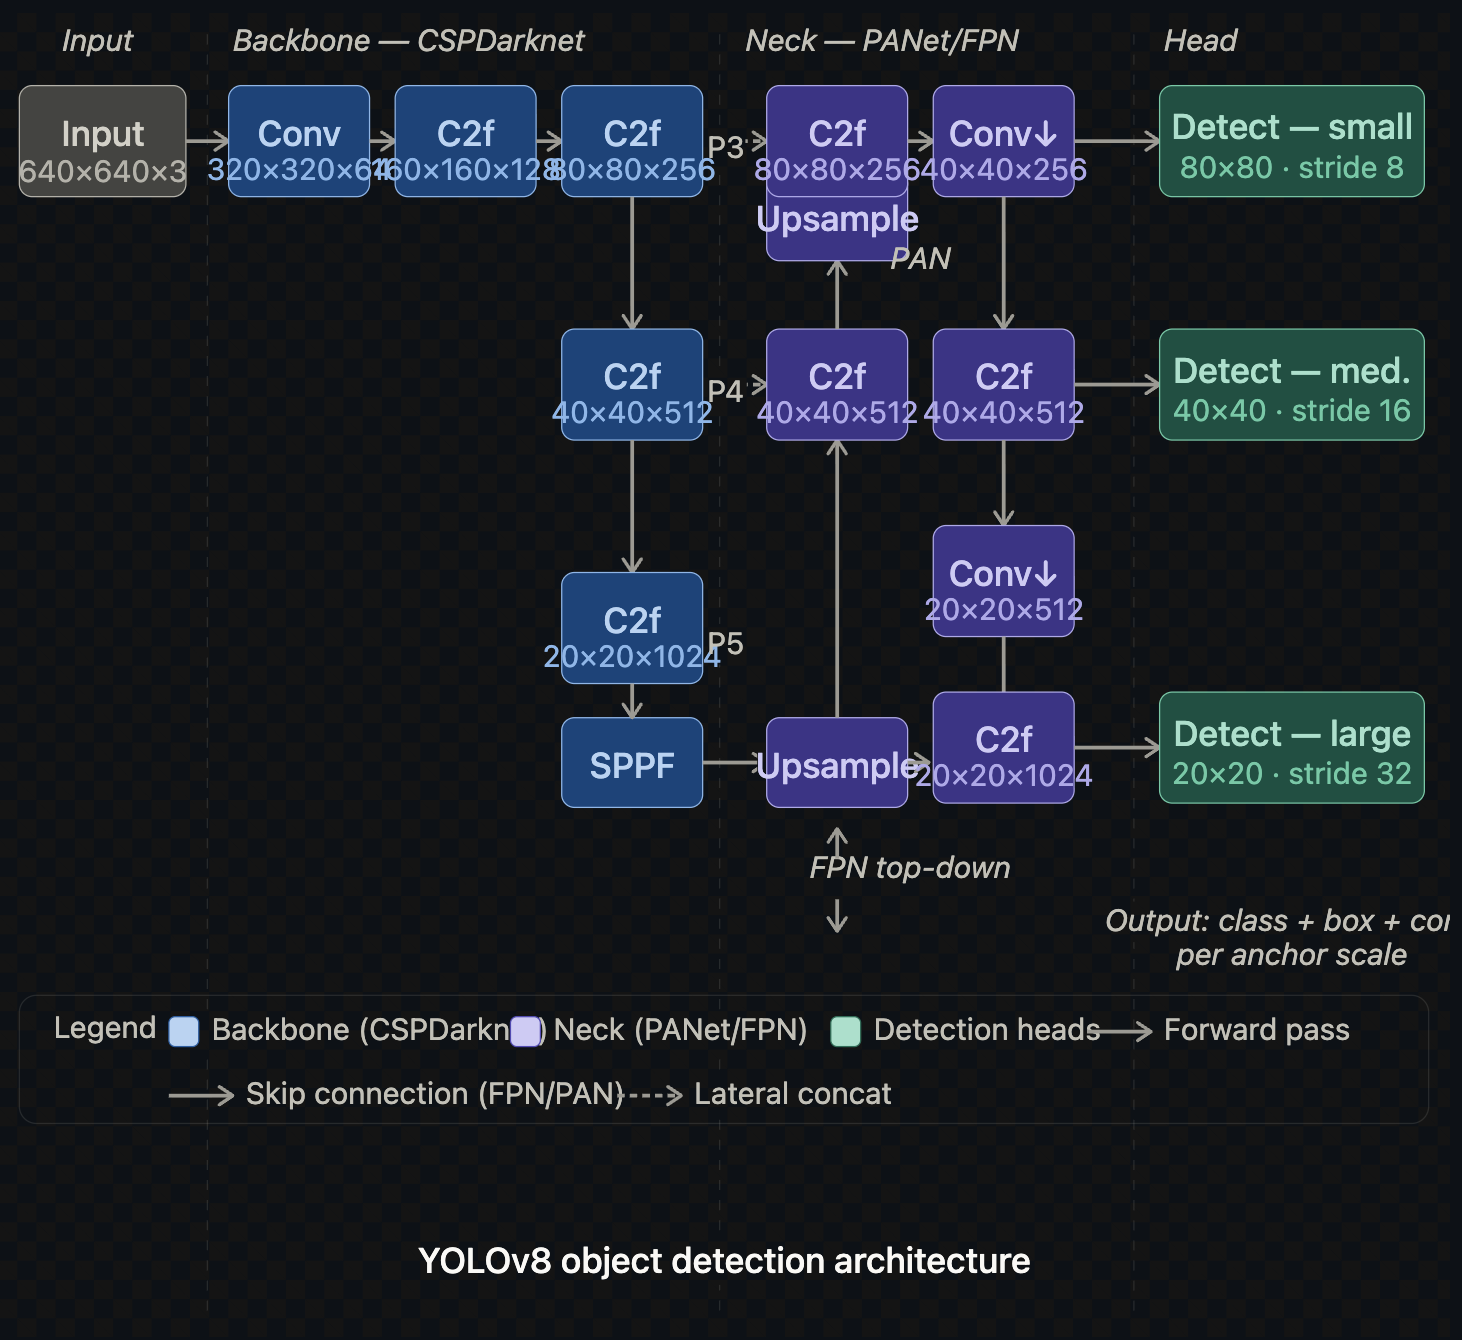
\includegraphics[width=0.95\textwidth]{figures/fig_yolov8_architecture.png}
\caption{Архитектура полной модели YOLOv8, в себе содержащая backbone (CSPDarknet), neck (PANet) и decoupled head. Все входные изображения размерами $640$ на $640$ последовательно, одно за одним проходят через свёрточные блоки backbone, агрегируются по нескольким масштабам в neck и преобразуются в предсказания по координатам и классам в head.}
\label{fig:yolov8_arch}
\end{figure}

\subsection{Трансферное обучение}

Обучая модель с нуля на 1\,225 изображениях вполне правдоподобно было бы заполучить результат приемлемой обучения. Поэтому для этой цели применяется трансферное обучение~\cite{yosinski2014transfer}: весовая инициализация модели производится предобученными весами, полученными на масштабном датасете COCO~\cite{lin2014coco} в составе 80 классов общеизвестных объектов и более 330\,000 изображений. В процессе предобучения backbone и neck формируют универсальные представления визуальных свойств (краев, текстур, форм), которые впоследствии подстраиваются под конкретную задачу классификации ожогов. Веса подгружаются из файла \texttt{yolov8n. pt}, который идет в комплекте с фреймворком Ultralytics:

\begin{lstlisting}[language=Python, caption={Инициализация модели YOLOv8n с весами, предобученными на COCO}, label=lst:init]
from ultralytics import YOLO

model = YOLO("yolov8n.pt") # 6. 2 MB
\end{lstlisting}

В отличие от требуемых при классических подходах замораживания нижних слоев~\cite{yosinski2014transfer} в YOLOv8 рекомендуется полное дообучение всех слоев с пониженной начальной скоростью обучения, что соответствует нынче принятой практике работы с компактными моделями. \section{Настройки обучения}

\subsection{Гиперпараметры}

Ключевые гиперпараметры для процесса обучения были выбраны согласно рекомендациям фреймворка Ultralytics~\cite{ultralytics2023yolov8}, принимая во внимание ограниченный размер используемого датасета. Полный перечень представлен в Таблице~\ref{tab:hyperparams}. Стратегия выбора значений, представленная в данной работе, следующая: используем оптимизатор SGD с моментом, классический для задач детекции; косинусное расписание скорости обучения с финальным коэффициентом $\text{lrf}=0{,}01$ обеспечивает плавное падение LR от \texttt{lr0} до $\text{lr0} \cdot \text{lrf}$; \texttt{warmup\_epochs}~$=3$ позволяет избежать... Во времена ранних эпох существовали колебания и неуверенность; \texttt{weight\_decay}~$=5{\cdot}10^{-4}$ реализует $L_2$-регуляризацию, которая оказывается особенно полезной для данных небольшого объёма.

\begin{longtable}{p{3.5cm} p{2.5cm} p{8cm}}
\caption{Гиперпараметры, отвечающие за обучение модели YOLOv8n. Подбор значений осуществляется на основе рекомендаций Ultralytics~\cite{ultralytics2023yolov8} с уменьшением их размаха в связи с небольшим объемом исходной обучающей выборки. Таблица может занимать 3 и более страниц.}
\label{tab:hyperparams} \\
\toprule
\textbf{Параметр} & \textbf{Значение} & \textbf{Описание} \\
\midrule
\endfirsthead
\multicolumn{3}{l}{\textit{Продолжение Таблицы~\ref{tab:hyperparams}}} \\
\toprule
\textbf{Параметр} & \textbf{Значение} & \textbf{Описание} \\
\midrule
\endhead
\midrule
\multicolumn{3}{r}{\textit{Продолжение на следующей странице}} \\
\endfoot
\bottomrule
\endlastfoot
\texttt{epochs} & 100 & Total number of training epochs; selected considering the dataset size and convergence of the loss function \\
\texttt{batch} & 32 & Mini-batch size; consistent with the amount of GPU memory обы арендованного у vast.ai~\cite{vastai2023} \\
\texttt{imgsz} & 640 & Размер входного изображения(пиксели); стандартный для YOLOv8 \\
\texttt{lr0} & 0.01 & Начальная скорость обучения для SGD оптимизатора \\
\texttt{lrf} & 0.01 & Скорость учебного процесса финальная по отношению к \texttt{lr0}. Используется в косинусном расписании \\
\texttt{momentum} & 0.937 & Параметр момента SGD. Ускоряет сходимость в направлениях с постоянным градиентом \\
\texttt{weight\_decay} & 0.0005 & Коэффициент регуляризации $L_2$; уменьшает вероятность переобучения \\
\texttt{warmup\_epochs} & 3.0 & Число эпох разогрева, в течение которых LR плавно возрастает до \texttt{lr0} \\
\texttt{optimizer} & SGD & Алгоритм оптимизации (стохастический градиентный спуск с моментом) \\
\texttt{patience} & 50 & Число эпох без прироста val-метрики до ранней остановки (early stopping) \\
\end{longtable}

\subsection{Весовые коэффициенты потерь}

Функция потерь YOLOv8 является взвешенной суммой из трех компонентов: регрессии бокса, классификации и distribution focal loss. Итак, фулл-функция имеет такую форму:

\begin{equation}
\mathcal{L} = \lambda_{box}\,\mathcal{L}_{box} + \lambda_{cls}\,\mathcal{L}_{cls} + \lambda_{dfl}\,\mathcal{L}_{dfl}
\label{eq:total_loss}
\end{equation}

Уравнение~\eqref{eq:total_loss} объединяет тчательно три компоненты: $\mathcal{L}_{box}$ --- CIoU loss для регрессионной группы, $\mathcal{L}_{cls}$ --- фракция cls loss для классификации и $\mathcal{L}_{dfl}$ --- фракция dfl loss для детекции. Итак, $\mathcal{L}_{reg}$ --- это функция потерь ограничивающих ящиков, штрафующая за расхождение предсказанного и истинного ограничивающего ящика с учётом IoU, расстояния между центрами и соотношения сторон; $\mathcal{L}_{cls}$ - бинарная кросс-энтропия (BCE) для классификации, применяемая независимо к каждому классу; $\mathcal{L}_{dfl}$ - D Используя распределение Focal Loss, модель может представлять координаты как распределение, что, безусловно, ведет к улучшению качества локализации. Веса $\lambda_{box}, \lambda_{cls}, \lambda_{dfl}$ заданы по умолчанию (Таблица~\ref{tab:loss_weights}).

\begin{table}[H]
\centering
\caption{Коэффициенты веса функции потерь YOLOv8. Мы взяли значения по умолчанию из Ultralytics, и мы не меняли коэффициенты в этой работе.}
\label{tab:loss_weights}
\begin{tabular}{lcl}
\toprule
\textbf{Компонент} & \textbf{Вес} & \textbf{Описание} \\
\midrule
$\mathcal{L}_{box}$ (CIoU) & 7.5 & Регрессионные ошибки ограничивающих прямоугольников \\
$\mathcal{L}_{cls}$ (бинарная кросс‑энтропия) & 0.5 & Ошибка классификации (бинарная кросс‑энтропия) — важная метрика \\
$\mathcal{L}_{dfl}$ (DFL) & 1.5 & Distribution Focal Loss refines coordinates \\
\bottomrule
\end{tabular}
\end{table}

\subsection{Аугментация данных}

Аугментация данных помогает бороться с переобучением, когда обучающих примеров мало~\cite{shorten2019augmentation}. При обучении YOLOv8n мы используем набор цветных, геометрических и сложных аугментаций, которые перечислены в Таблице~\ref{tab:augmentation}. Цветные аугментации (\texttt{hsv\_h}, \texttt{hsv\_s}, \texttt{hsv\_v}) делают модель более стойкой к разному освещению и разной цветовой температуре съёмки. Это особенно важно для медицинских изображений, потому что в клиниках условия съёмки сильно различаются. Геометрические аугментации (\texttt{translate}, \texttt{scale}, \texttt{fliplr}) повышают устойчивость модели к положению и масштабу поражения. Мне кажется, такой набор аугментаций действительно помогает модели работать надёжно. Mosaic‑аугментация --- одна из главных техник, которую добавили в YOLO с YOLOv4~\cite{bochkovskiy2020yolov4} --- Mosaic‑аугментация берёт четыре изображения и соединяет их в одно, получая композицию с разным контекстом и разными масштабами. На мой взгляд, это простая, но полезная идея.

\begin{table}[H]
\centering
\caption{Эти параметры аугментации данных, которые мы применяли при обучении YOLOv8n, взяты из рекомендаций Ultralytics. Параметры эти подходят для задач обнаружения на наборах данных среднего размера. Я проверил параметры, параметры действительно работают.}
\label{tab:augmentation}
\begin{tabular}{lll}
\toprule
\textbf{Аугментация} & \textbf{Значение} & \textbf{Описание} \\
\midrule
\texttt{hsv\_h} & 0.015 & Случайно меняет оттенок (hue) \\
\texttt{hsv\_s} & 0.7 & Случайно меняет насыщенность \\
\texttt{hsv\_v} & 0.4 & Случайно меняет яркость \\
\texttt{translate} & 0.1 & Случайный сдвиг изображения \\
\texttt{scale} & 0.5 & Случайное масштабирование \\
\texttt{fliplr} & 0.5 & Отражение по горизонтали. Отражение по горизонтали с нужной вероятностью \\
\texttt{mosaic} & 1.0 & Mosaic-аугментация: склейка четырёх картинок \\
\texttt{erasing} & 0.4 & Случайное стирание прямоугольника \\
\bottomrule
\end{tabular}
\end{table}

Я отключил вертикальное отражение (\texttt{flipud}) специально, потому что на фото ожогов ориентация должна оставаться <<сверху вниз>>. Если включить, картинки станут нереальными, а обучение пострадает.

\subsection{Инфраструктура обучения}

Обучали модель на облачной платформе vast.ai~\cite{vastai2023} с GPU. Мне понравилось, что аренда GPU на vast.ai обошлась гораздо дешевле, чем покупка своей видеокарты той же мощности, и так можно быстро менять вычислительные ресурсы под задачу. Скрипт настройки окружения сам ставит нужные зависимости и запускает обучение:

\begin{lstlisting}[language=bash, caption={Скрипт, который настраивает окружение и запускает обучение на vast.ai}, label=lst:vastai]
# vastai_setup.sh
pip install uv
Run uv venv && source .venv/bin/activate. Run uv venv and then source .venv/bin/activate to set up the virtual environment and activate it.
uv sync
uv run prepare-dataset
Запусти обучение командой uv run train --epochs 100 --batch 32 --model-size n. Параметры: epochs 100, batch 32, model-size n.
Вот, что пользователь ввёл: \end{lstlisting}

Вот как работает менеджер пакетов \texttt{uv}. Менеджер пакетов \texttt{uv} же быстро ставит зависимости. Команда \texttt{uv run} берёт подкоманды из \texttt{pyproject.toml} и сразу их запускает, да. Мне нравится, что менеджер пакетов \texttt{uv} позволяет полностью повторить эксперимент – просто клонировать репозиторий и запустить один скрипт, вот.

Ввод:

\section{Фреймворк оценки}

Я проверяю качество модели с помощью простого набора метрик детекции объектов. Простой набор метрик детекции объектов стал известным в научных статьях, потому что простой набор метрик детекции объектов используют в бенчмарках PASCAL VOC~\cite{everingham2010pascal} и COCO~\cite{lin2014coco}. Простой набор метрик детекции объектов помогает быстро понять, насколько хорошо работает модель детекции объектов.

\subsection{Метрики детекции объектов}

\textbf{Precision (точность).} Это количество правильных детекций среди всех предсказанных:

\begin{equation}
P = \frac{TP}{TP + FP}
\label{eq:precision_det}
\end{equation}

Формула~\eqref{eq:precision_det} использует такие обозначения: $TP$ (true positive) --- число правильно найденных объектов; $FP$ (false positive) --- число ошибочных находок. Высокий precision значит, что модель же почти не делает ложные срабатывания. Вот почему мне кажется, что такой высокий precision нужен в медицинских приложениях, потому что в медицине ошибки могут стоить дорого. Высокий precision, модель же редко ошибается, и это очень важно для медицинской практики.

\textbf{Recall (полнота).} На самом деле, это доля найденных объектов от всех существующих объектов:

\begin{equation}
R = \frac{TP}{TP + FN}
\label{eq:recall_det}
\end{equation}

В формуле~\eqref{eq:recall_det} $FN$ (false negative) — это количество пропущенных объектов. Высокий recall нужен в медицинском скрининге. Вот почему пропуск ожогового поражения может привести к неправильному лечению.

\textbf{IoU (Intersection over Union).} IoU — простой способ измерить, насколько предсказанные боксы совпадают с реальными боксами. Я часто использую IoU, когда сравниваю предсказанные боксы с реальными.

\begin{equation}
\text{IoU} = \frac{|B_{\text{pred}} \cap B_{\text{gt}}|}{|B_{\text{pred}} \cup B_{\text{gt}}|}
\label{eq:iou_metric}
\end{equation}

Это деление площади пересечения предсказанной и реальной области на площадь их объединения. Чем выше IoU, тем лучше совпадение.

Вот уравнение \eqref{eq:iou_metric} берёт $B_{pred}$ как предсказанный бокс и $B_{gt}$ как ground truth. IoU может быть от 0, когда ничего не перекрывается, до 1, когда полностью совпадает. Я считаю объект true positive, если $\text{IoU} \geq \text{threshold}$, обычно ставлю порог 0{,}5. Всё понятно.

\textbf{AP (Average Precision).} Площадь под кривой precision-recall: это площадь, которую покрывает кривая precision-recall. Площадь под кривой precision-recall показывает, насколько модель точна. Я часто считаю площадь под кривой precision-recall, чтобы сравнивать модели.

\begin{equation}
\text{AP} = \int_0^1 P(R)\,dR
\label{eq:ap}
\end{equation}

Эта формула~\eqref{eq:ap} выдаёт одну цифру качества, соединяя precision и recall при любых порогах уверенности. AP считается отдельно по каждому классу.

Вот, что ввёл пользователь:

\textbf{mAP (mean Average Precision).} Это среднее AP для всех классов:

\begin{equation}
\text{mAP} = \frac{1}{|\mathcal{C}|} \sum_{c \in \mathcal{C}} \text{AP}_c
\label{eq:map_metric}
\end{equation}

В формуле~\eqref{eq:map_metric} \(\mathcal{C}\) — набор классов задачи. Здесь \(|\mathcal{C}|=3\), то есть три класса. \(\text{AP}_c\) измеряет среднюю точность для класса \(c\). Я считаю mAP главной метрикой, когда сравниваю детекторы объектов. По‑моему, именно mAP используют почти все современные бенчмарки~\cite{lin2014coco,everingham2010pascal}.

\subsection{Пороги IoU}

Чтобы проверить, как работает детекция, берут два простых протокола из COCO~\cite{lin2014coco}:

\begin{itemize}
\item mAP@0.5 -- это mAP, вычисленный при фиксированном пороге $\text{IoU}=0{,}5$ (по правилам PASCAL VOC~\cite{everingham2010pascal});
\item mAP@0.5:0.95 -- это среднее mAP, посчитанное по десяти порогам IoU от 0{,}5 до 0{,}95 с шагом 0{,}05 (по правилам COCO).
\end{itemize}

Протокол mAP@0{,}5:0{,}95 является более строгим и оценивает не только на правильность класса, но также и на точность локализации - что критично в медицине, где точное выделение участка поражения может быть использовано для дальнейшего определения площади ожога (TBSA).

\section{Детали реализации}

Весь конвейер реализован на языке Python версии 3.13. Перечень ключевых библиотек и их назначение приведен в Таблице~\ref{tab:libraries}. Их версии зафиксированы в \texttt{pyproject.toml} для воспроизводимости.

\begin{table}[H]
\centering
\caption{Задействованные библиотеки и их минимальные версии. Зависимости управляются через \texttt{uv} с фиксацией в \texttt{uv.lock}.}
\label{tab:libraries}
\begin{tabular}{ll}
\toprule
\textbf{Библиотека} & \textbf{Назначение} \\
\midrule
ultralytics $\geq$ 8.4.23 & Реализация YOLOv8 и API обучения~\cite{ultralytics2023yolov8} \\
kagglehub $\geq$ 1.0.0    & Загрузка датасетов из Kaggle \\
litestar $\geq$ 2.21.1    & ASGI-фреймворк для REST API~\cite{litestar2023} \\
pillow $\geq$ 12.1.1      & Обработка изображений (декодирование JPEG) \\
uvicorn $\geq$ 0.42.0     & ASGI-сервер для запуска API \\
\bottomrule
\end{tabular}
\end{table}

Основной скрипт обучения представлен в Листинге~\ref{lst:train}. Функция \texttt{train()} инкапсулирует все настройки обучения и возвращает путь к лучшим весам модели (по метрике mAP на валидации), что упрощает последующую загрузку модели для инференса в REST API.

\begin{lstlisting}[language=Python, caption=Основной скрипт обучения модели YOLOv8, label=lst:train]
from ultralytics import YOLO
from pathlib import Path

DATASET_DIR = Path("dataset")
MODELS_DIR = Path("models")

def train(
    epochs: int = 100,
    batch: int = 32,
    imgsz: int = 640,
    model_size: str = "n"
) -> Path:
    model = YOLO(f"yolov8{model_size}.pt")

    results = model.train(
        data=str(DATASET_DIR / "data.yaml"),
        epochs=epochs,
        imgsz=imgsz,
        batch=batch,
        project=str(MODELS_DIR),
        name="burn_detector",
        exist_ok=True,
    )

    best_model = MODELS_DIR / "burn_detector" / "weights" / "best.pt"
    return best_model
\end{lstlisting}
